% This document is under the terms of the GPL Licence.
%
% Create DVI:
% latex sqltools_tutorial_en.tex
% Show DVI:
% yap sqltools_tutorial_en.dvi
% Create PDF:
% dvipdfm sqltools_tutorial_en.dvi
%

\documentclass[a4paper,titlepage]{article}
\hoffset = -2cm
\voffset = -2cm
\addtolength{\textwidth}{4cm}
\addtolength{\textheight}{4cm}

\usepackage{graphicx}
\DeclareGraphicsExtensions{.jpg,.jpeg,.gif}

\author{Drzewiecki Tomasz}
\title{SQLTools in 5 steps\\ver. 0.1}

\begin{document}
\maketitle
\tableofcontents
\newpage

\section{Connecting}
Let's start by executing the program. We'll see the database connection window.\\
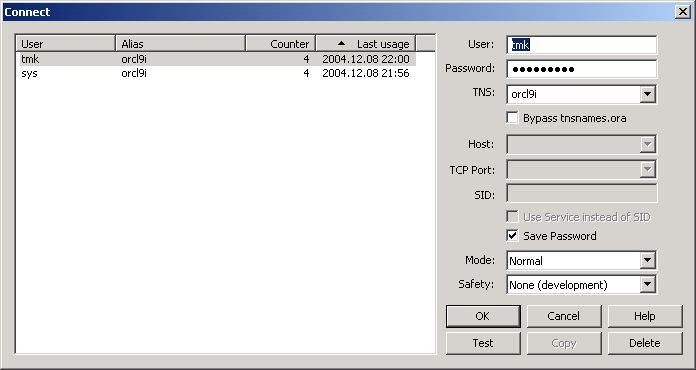
\includegraphics[bb=0 0 696 370,width=\textwidth]{00login00}
On the left side there is a list with previous connections to different databases. In the picture, the list is ordered 
by the last usage time, but we can sort the list by any of columns.  Double-click on one of the connections to reestablish it.

To connect to a new database, enter user name and 
password, and then choose a database name from the TNS list (to be more precise - list of SIDs). 

What if we don't have an incorrect \emph{tnsnames.ora} file, or none at all? 
We can enter parameters manually! Check the \emph{Bypass tnsnames.ora} option, and enter the computer name (or IP), 
database, and connection port (typically 1521).\\
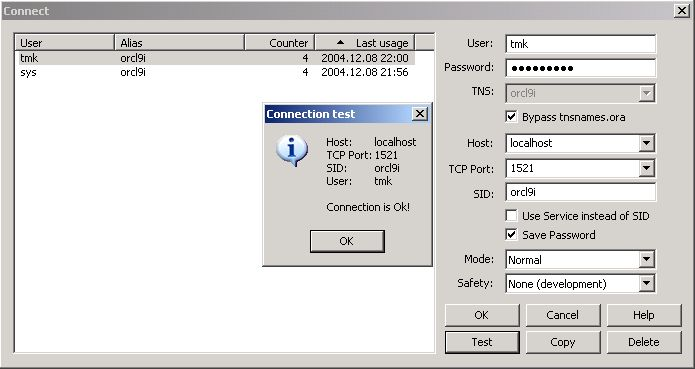
\includegraphics[bb=0 0 695 369,width=\textwidth]{00login01}

The \emph{Test connection} button is very useful during connection attempts. It checks the existence of an Oracle instance and the 
correctness of the login information, but does not log on to the database.

If it is necessary to log as a SYSDBA or a SYSOPER to do administration tasks, select the appropriate option
under the \emph{Mode} dropdown list.\\
\begin{center}
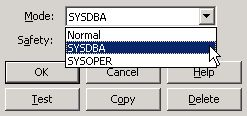
\includegraphics[bb=0 0 247 116,scale=.7]{00login02}
\end{center}

After logging on to the database, we see current connection parameters and 2 buttons on the toolbar. 
Those buttons allow us to disconnect, connect to another Oracle instance, or log on as an another user.\\
\begin{center}
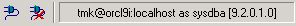
\includegraphics[bb=0 0 296 26,scale=.7]{00login03}
\end{center}

%\newpage
\section{Main window}

Here is the main window of the program.\\
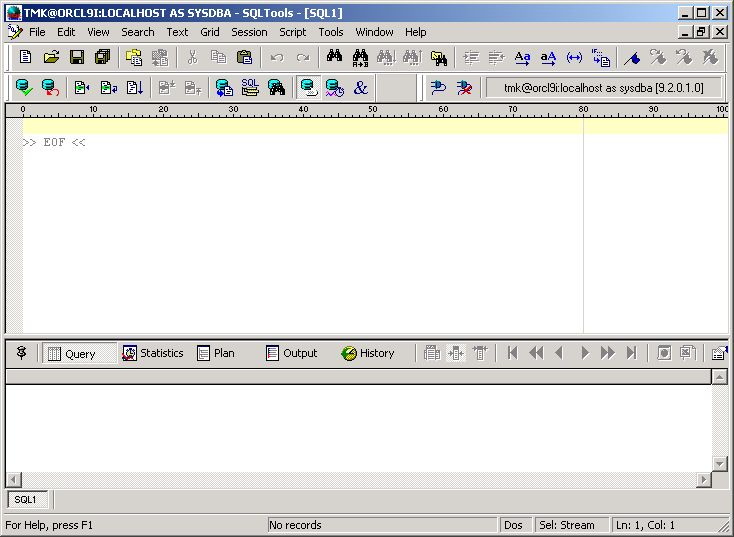
\includegraphics[bb=0 0 734 537,width=\textwidth]{01main00}

In the editor we can execute SQL, packages, procedures and triggers.
The lower window contains query results. Let's do a simple experiment. In the upper window, type:
\begin{center}
SELECT 5+10 FROM DUAL;\\
\end{center}
Press \textbf{F5}. We can see  the result below!\\
\begin{center}
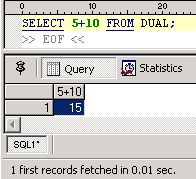
\includegraphics[bb=0 0 196 179,scale=.7]{01main01}
\end{center}

Let's try something more complicated.
\begin{center}
SELECT * FROM user\_tables;
\end{center}

Notice that if we type in lowercase, SQL keywords are changed to uppercase as we type. 
It is automatically formatted. The menu option \emph{Tools $\to$ Application/Editor Settings $\to$ 
Normalize keywords} controls this feature.  If an unformatted piece of code is in the window, 
we can 'beautify' it by choosing the 
menu command \emph{Text $\to$ Normalize Keyword}.

Let's execute the above query by pressing \textbf{F5}. Depending on the contents of USER\_TABLES, we will probably see a 
dozen or so rows in the result set.\\
\begin{center}
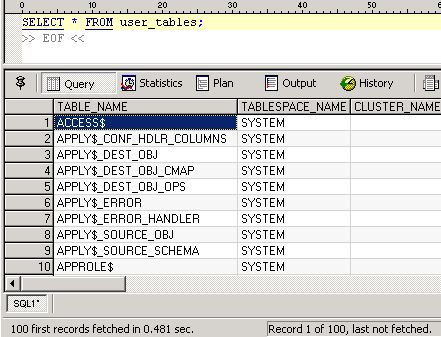
\includegraphics[bb=0 0 441 337,scale=.7]{01main02}
\end{center}
In the picture, the bottom status line tells us that the program got only the first 100 rows in 0.481s.  More rows will
be fetched if we scroll to the bottom of the results.
The number of rows fetched can be changed by the menu option
\emph{Tools $\to$ Session/DDL/Grid Settings $\to$ Data Grid $\to$ Row prefetch}.

Let's choose menu option \emph{Session $\to$ Enable Session Statistics}. Execute the same query again.  Now click on the second tab \emph{Statistics}.\\
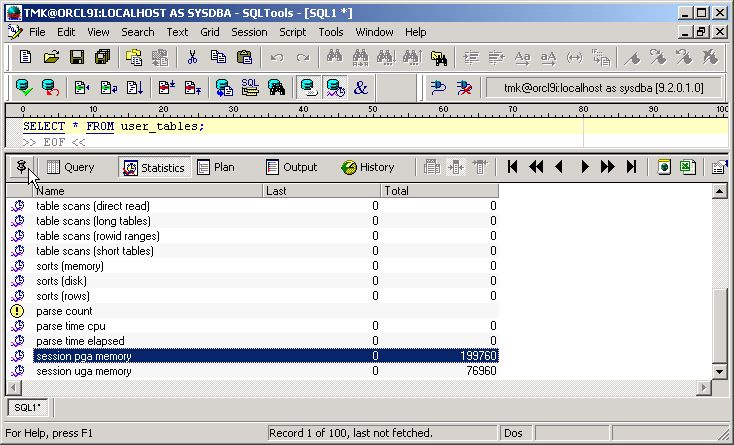
\includegraphics[bb=0 0 734 445,width=\textwidth]{01main03}

On this tab we see the statistics for the last query.  (We would see statistics for the entire session, but we've only run one query since we started collecting statistics.)  In the picture, the mouse pointer is located over a very useful 
button - Disable auto switching panes. By default, the \emph{Query} tab will automatically reopen if we execute another query. 
Let's press \textbf{F5} to see this behavior. Now go to the \emph{Statistics} tab again and click the button. Press \textbf{F5} again. What is the result?

Turn off Disable auto switching panes button and press \textbf{F9}. The query execution plan will be displayed in the \emph{Plan} tab.\\
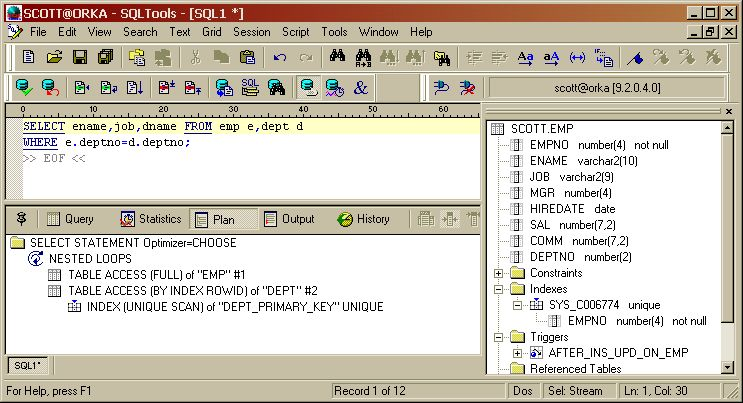
\includegraphics[bb=0 0 743 403,width=\textwidth]{01main04}

Back in the upper window, click anywhere inside the word 'USER\_TABLES'. Press \textbf{F12}.\\
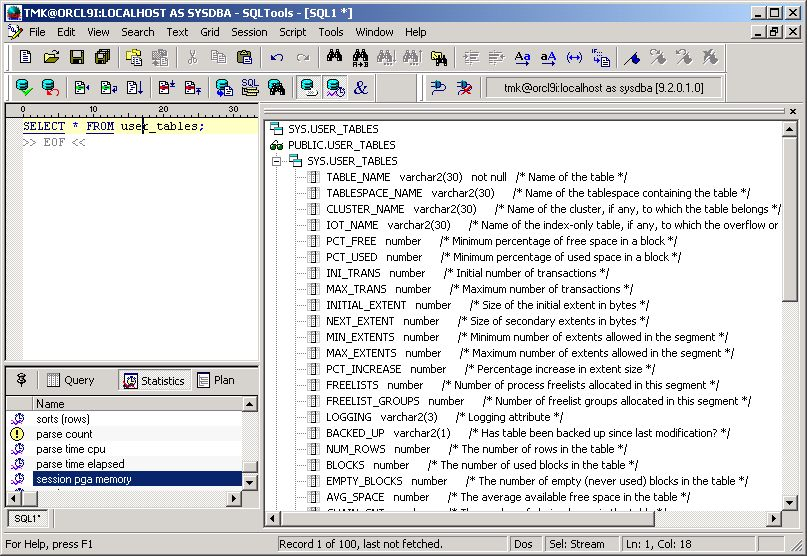
\includegraphics[bb=0 0 807 556,width=\textwidth]{01main05}

This brings up a window describing the structure of the table or view. We can also see the list of objects that depend on this table or view, and the list of objects from which the table or view is constructed. This is a very useful tool for quickly researching the dependencies between objects.\\
\begin{center}
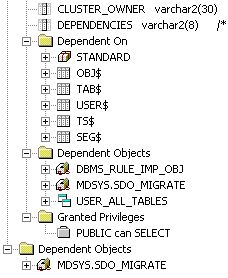
\includegraphics[bb=0 0 228 278,scale=.7]{01main06}
\end{center}

%\newpage
\section{Object list}
Press \textbf{Alt+3} when the cursor is inside the editor. This opens the object browser.\\
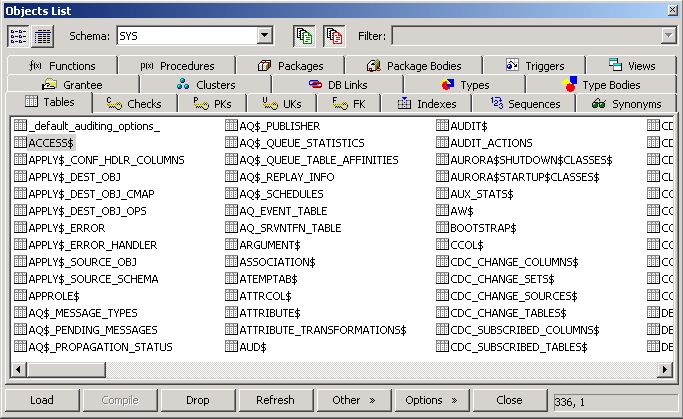
\includegraphics[bb=0 0 683 419,width=\textwidth]{02objview00}

This window lists all the objects in our schema. Let's select any table (on the \emph{Tables} tab), for example COUNTRIES from the HR schema. Rightclick on it and select \emph{Query}.\\
\begin{center}
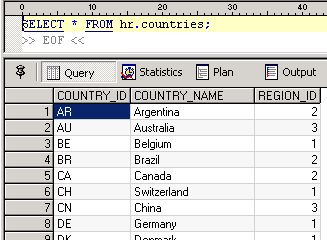
\includegraphics[bb=0 0 327 240,scale=.7]{02objview02}
\end{center}

We have created a new editor window and executed the query:
\begin{center}
SELECT * FROM hr.countries;
\end{center}

Choose the same object in the object list (\textbf{Alt+3}) and select the \emph{Load} option from the menu (or simply doubleclick it). We see the \emph{Local DDL Preferences} window.  Select the options as shown in the picture, and then press OK.
\begin{center}
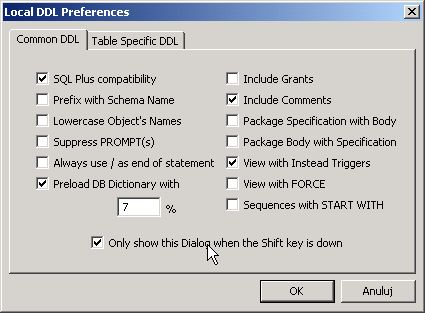
\includegraphics[bb=0 0 425 313,scale=.7]{02objview01}
\end{center}

A new editor window appears, with the script to create the table.  This works with other objects, as well.\\
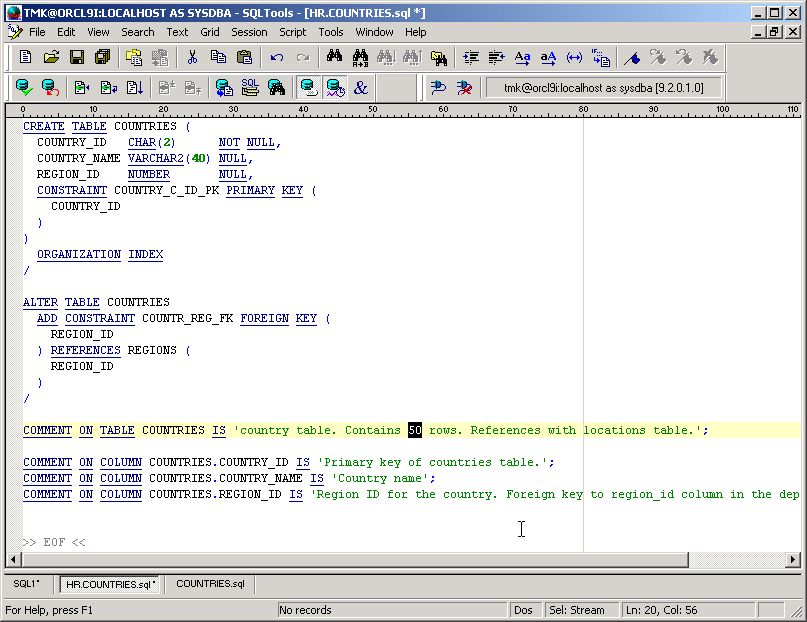
\includegraphics[bb=0 0 807 622,width=\textwidth]{02objview03}

This makes it simple to recreate the object.
For example, change something minor, such as the description of one column, and then press \textbf{F5}. If you have no errors, the changes will be made in the database. The \emph{Output} tab will show script execution errors with a red icon, and the results of successful commands with a blue icon.
\begin{center}
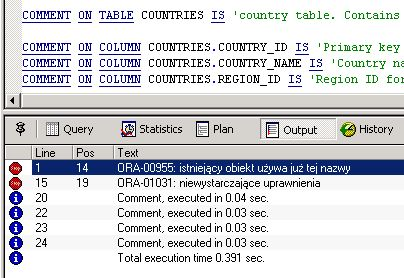
\includegraphics[bb=0 0 404 278,scale=.7]{02objview04}
\end{center}

One very useful option of the \emph{Object list} is the ability to load many objects (for example packages) into the editor at once, as a one big script. For example, select some package bodies and choose \emph{Load all in one} from the rightclick menu.\\
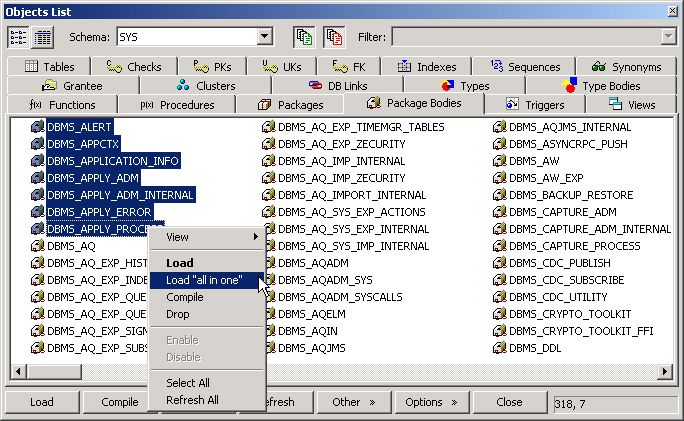
\includegraphics[bb=0 0 684 421,width=\textwidth]{02objview05}

A new editor window appears, with a defining script for the selected package bodies. One possible use for this feature is to search all packages to find a particular error message.

\section{The exercises never will be enough}
One of the beauties of SQLTools (apart from its price) is that it isn't dominated by wizards and magic buttons. Trust me, even for complex developement projects, this spartan environment is enough. 

Enough chattering - let's do some exercises! Suppose that we are on Oracle8i or above, and we have rights to create objects, drop objects, and execute all other operations on objects in our schema.

\subsection{Do these exercises}
\begin{enumerate}
\item Create a table like USER\_TABLES, but with only the first three columns.
\item Copy data to the new table, using an INSERT from USER\_TABLES.
\item Create your own package with one public procedure typing one line (using 'put'+CTRL+SPACE - type word \emph{put} and press $<$CTRL+SPACE$>$).  The output should be data extracted from the new table.
\item Create a standalone procedure which will call the procedure from your package.
\item Create unnamed body:\\
\indent BEGIN\\
\indent \indent our\_created\_procedure;\\
\indent END;
\item Execute the script pressing \textbf{F5}. Save the script to the file.
\item Select the table name in the editor and press the \textbf{F12}. On what objects does it depend? What objects use this table?
\item Close everything. Open the object list again (\textbf{Alt+3}). Drop the new table using the button.
\item Enter the object list on the \emph{Package bodies} tab. Press the \emph{Refresh} button, and watch what is displayed on the left side of the package. 
\item Enter the editor and load the script. Let's try to execute it. Why it doesn't succeed?
\item Finally, return to the object list, and drop the procedure and the package. You have finished!
\end{enumerate}

\subsection{Hints (of course there are many ways to reach the same goal)}
1. CREATE TABLE \dots\ AS SELECT table\_name, tablespace\_name, cluster\_name FROM user\_tables WHERE 1=0;\\[.3cm]
2. INSERT INTO \dots\ SELECT \dots;\\[.3cm]
3. Open the object list, load any package (specification + body for simple), remove all but 1 procedure and add there three lines:
\begin{itemize}
\item with variable(s) declaration;
\item with SELECT \dots\ INTO \dots;
\item with Dbms\_Output.Put\_Line();
\end{itemize}
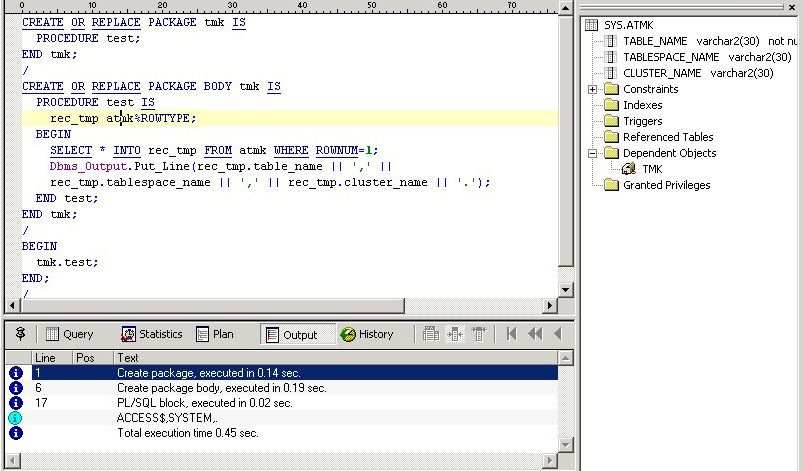
\includegraphics[bb=0 0 803 471,width=\textwidth]{04exercise00}
4,5,6,7. An example implementation.\\
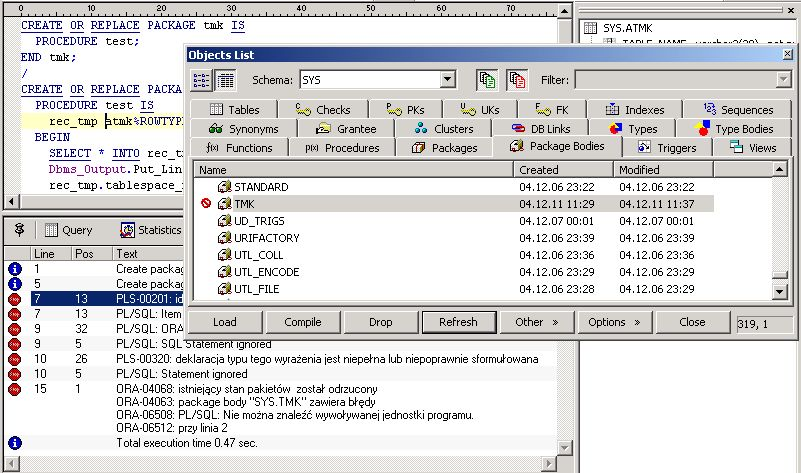
\includegraphics[bb=0 0 803 473,width=\textwidth]{04exercise01}
8,9. Mark at the 'invalid' package and error messages in a polish language.

\section{Advanced topics - customizing SQLTools settings}
Why dwell on this matter? We have options in the menu:
\begin{itemize}
\item \emph{Text $\to$ File Settings \& Information}
\item \emph{Tools $\to$ Session / DDL / Grid Settings}
\item \emph{Tools $\to$ Application / Editor Settings}
\end{itemize}
Keyboard shortcuts can be changed in the file \emph{Data / custom.keymap}.

\subsection{And what next?}
\emph{2004-12-13}
At this moment, the program isn't modular - it consists of one big *.exe file. In the future we are looking at the idea of plugins, which everybody can create without looking at the main source.

Both SQLTools and OpenEditor (which represents the bulk of the SQLTools code) have been recently been made available as projects on SourceForge. We hope that this will lead to 'big jump' in developement of the program.

We hope that everybody that reads this will support our development team, even if it is only in small things such as testing new releases and supporting bugs. We will be very grateful!

\end{document}

